%% ------------------------------------------------------------------------- %%
\chapter{Aplicação}
\label{cap:aplicacao}

Como dito no capítulo \ref{cap:desenvolvimento}, utilizamos o site GuiaFolha como nosso estudo de caso. Escolhemos esse sistema por ter dados de fácil extração. No entanto, a base de dados da aplicação \emph{LookingFor} \cite{Repo} pode ser estendida, recebendo outras fontes de dados. Bastaria adaptar os dados de cada fonte ao nosso modelo, que já foi apresentado.

No site GuiaFolha, estão catalogados cerca de 950 restaurantes da cidade de São Paulo. Muitos desses sites não possuem endereços eletrônicos associados, apenas uma breve descrição. Outras informações são apresentadas de forma estruturada, como tipo de cozinha, endereço, telefone, preço médio e o horário de funcionamento. O formulário de busca desse site pode ser visto na figura \ref{fig:form}. O usuário consulta o sistema utilizando um campo de texto e algumas caixas de seleção.

% figura
\begin{figure}[!h]
  \centering
  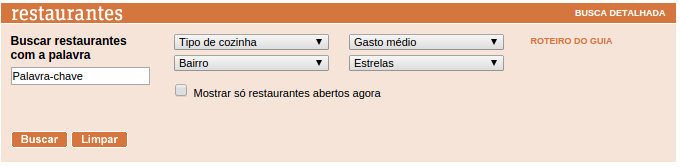
\includegraphics[width=\textwidth]{GuiaFolha-Formulario.png} 
  \caption{Formulário de restaurantes do site GuiaFolha.}
  \label{fig:form} 
\end{figure}

Para simplificar o nosso estudo, unimos o tipo de cozinha e a descrição para formar o corpo do documento. Os outros dados foram armazenados como metadados. 

No aplicativo \emph{LookingFor}, também fornecemos uma caixa de texto para o usuário expressar a sua necessidade. No entanto, trocamos as caixas de seleção ``gasto médio'', ``bairro'' e ``estrelas'' pelos botões ``preço'', ``distância'' e ``qualidade'', respectivamente. Com isso, simplificamos a interface de busca, mantendo certa liberdade. Esperamos que esse novo formato torne a formulação das consultas mais rápida e menos frustrante para o usuário.

Apresentamos esse aplicativo para um grupo de 19 usuários, guardando alguns dados sobre os seus acessos. Além disso, pedimos que eles respondessem um breve questionário, relatando a sua experiência.

% %% ------------------------------------------------------------------------- %%
\section{Resultados}
\label{sec:resultados}

Utilizamos um sistema de gerenciamento de banco de dados para guardar as informações dos acessos dos usuários. O software MySQL foi escolhido por termos maior familiaridade. Duas tabelas foram criadas: buscas e escolhas.

A tabela ``buscas'' foi usada para registrar as consultas feitas no sistema. Nela estão quatro colunas principais: \emph{text}, \emph{distance}, \emph{price}, \emph{grade}. A coluna \emph{text} representa os termos da consulta, como digitados pelo usuário. As outras três colunas guardam as prioridades dos parâmetros da busca. Essas colunas terão valor nulo se não forem escolhidos pelo usuário. Caso contrário, terão como valor um número natural menor ou igual ao número total de parâmetros.

A outra tabela, ``escolhas'', guarda a posição do resultado escolhido por um usuário. Partimos da hipótese que, quando um usuário clica em algum resultado, então este pode ser interessante. Não necessariamente esse interesse se traduz em relevância, mas pode ser um indicador. Algumas evidências presentes nesses resultados podem contribuir para entendermos o que o usuário necessita.

Para registrar essa escolha, apenas uma coluna é utilizada, chamada ``posição''. Quanto mais próximo o resultado está do topo da lista de resultados, melhor é a sua colocação. Ou seja, maior foi a pontuação dada pelo sistema de RI. Se muitos usuários escolhem resultados longe do topo, isso pode indicar falhas no nosso sistema de ranqueamento.

% %% ------------------------------------------------------------------------- %%
\subsection{Consultas}
\label{subsec:consultas}

Nesse período de testes, 253 consultas foram realizadas. Em média 11,8 consultas por usuário. Muitos termos foram repetidos nas consultas, de forma que apenas 87 distintas foram feitas, des-considerando os parâmetros escolhidos. Dessas, 40 (46\%) não retornaram nenhuma resposta.

Duas hipóteses podem ser feitas sobre esse fato. Primeiro, por termos usado a descrição breve dos estabelecimentos do site GuiaFolha, o dicionário do sistema foi construído com poucos termos. Segundo, por termos usado o modelo saco-de-palavras sem nenhum processamento linguístico, muitos termos próximos não foram associados durante a busca. Por exemplo, a consulta ``japonesa'' retorna 27 resultados, mas ``japonês'' não retorna nenhum. É importante para um sistema de RI compreender a linguagem utilizada pelos seus usuários, para que possa satisfazer a necessidade de informação sem um maior esforço por parte do usuário.

Considerando os parâmetros utilizados nas consultas, podemos entender que aspectos dos estabelecimentos interessam mais os usuários. A frequência de cada parâmetro pode ser vista na figura \ref{fig:graffreqpar}. Cada barra é segmentada pela colocação do parâmetro na ordem de prioridade.

% figura
\begin{figure}[!h]
  \centering
  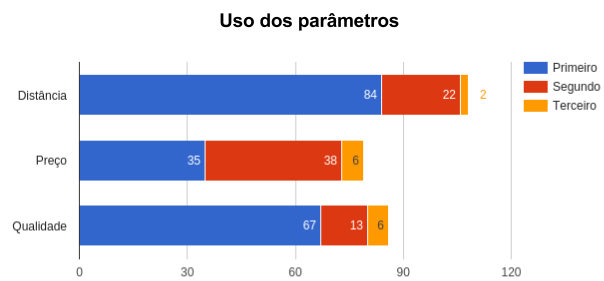
\includegraphics[width=0.8\textwidth]{Grafico-parametros.png} 
  \caption{Gráfico da frequência dos parâmetros nas consultas.}
  \label{fig:graffreqpar}
\end{figure}

O parâmetro distância foi o mais utilizado, estando presente em 108 consultas. Uma diferença de 20,4\% para o segundo colocado. No entanto, isso não quer dizer que os usuários tenham uma maior necessidade por estabelecimentos próximos ao seu local. A interface de usuário do aplicativo apresenta um mapa a todo momento, mesmo antes dos resultados da busca serem apresentados. Isso pode estimular o usuário a fazer consultas com conceitos geográficos, como a distância.

O preço foi o menos comum dos parâmetros, mas foi o mais utilizado como segundo na ordem de prioridade. Essa pode ser uma necessidade menor do usuário, mas ainda é um parâmetro relevante.

Todos os três parâmetros foram usados poucas vezes no final da ordem de prioridade. Podemos ver isso também na figura \ref{fig:grafnumpar}, a qual mostra o número de parâmetros por consulta. 94,5\% delas utilizaram até dois parâmetros. Considerando a distribuição das frequências na figura anterior, entendemos que os três parâmetros são relevantes para os usuários, mas não todos ao mesmo tempo.

% figura
\begin{figure}[!h]
  \centering
  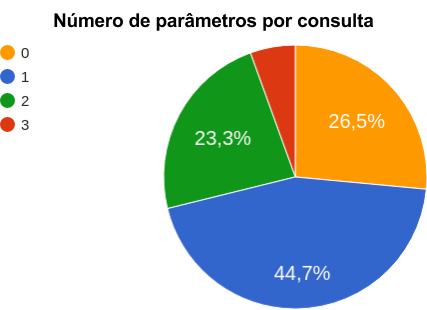
\includegraphics[width=0.50\textwidth]{Grafico-parametrosPorConsulta.png} 
  \caption{Gráfico do número de parâmetros por consulta.}
  \label{fig:grafnumpar}
\end{figure}

Já que os usuários foram introduzidos ao aplicativo para realizar este experimento, provavelmente tentaram entender o sistema de busca e o significado de cada parâmetro no primeiro momento. Para isso, realizaram consultas semelhantes, comparando seus resultados. Isso pode explicar a grande proporção de consultas com apenas um deles selecionado. Para resultados mais conclusivos, seria necessário expôr os usuários ao aplicativo por um tempo maior, deixando-os se familiarizar com as funcionalidades.

% %% ------------------------------------------------------------------------- %%
\subsection{Estabelecimentos escolhidos}
\label{subsec:estabescol}

Rastreando os cliques feitos na lista de estabelecimentos do aplicativo, foi possível guardar a posição do elemento escolhido. Contudo, no período de testes, apenas 39 desses cliques foram feitos. Isso representa 24,5\% das 163 buscas com algum resultado.

Como já foi dito, os usuários não acessaram o \emph{LookingFor} por conta própria, mas foram convidados a fazê-lo. É possível que para esse grupo não houvesse uma real necessidade das informações que o aplicativo pode prover, estando mais preocupados em explorar a interface de usuário, gerando poucos cliques na lista de resultados.

Como pode ser visto na figura \ref{fig:freqcliq}, 17 dos 39 estabelecimentos escolhidos estavam no topo da lista, e existe uma preferência pelos primeiros resultados.

O aplicativo retornou em média 18,4 resultados por busca, considerando apenas as que retornaram algo. Se esse número fosse menor, poderíamos argumentar que as posições mais baixas tiveram uma frequência maior por serem as únicas possíveis na maioria dos casos.

% figura
\begin{figure}[!h]
  \centering
  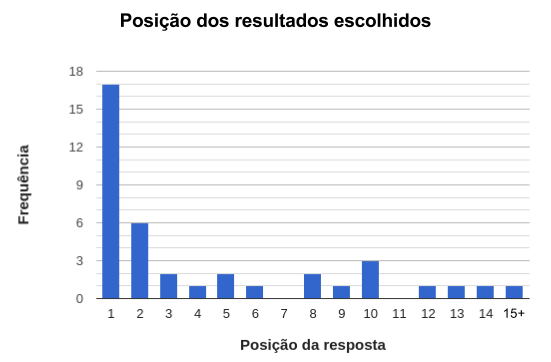
\includegraphics[width=0.5\textwidth]{Grafico-escolhas.png} 
  \caption{Frequência de cliques por posição da resposta.}
  \label{fig:freqcliq}
\end{figure}

A posição média dos estabelecimentos escolhidos é 4,5. Em um monitor 1680x1050, a lista de resultados mostra entre 4 e 5 elementos, sem rolagem. Portanto, os usuários podem ter clicado nesses primeiros por estarem visíveis. Além disso, uma posição é sempre menor ou igual ao tamanho da lista, logo, os números menores estarão em mais listas. A primeira posição, por exemplo, está em todas.

Como foi dito antes, com um período de testes mais longos conseguiríamos avaliar melhor a reação dos usuários ao aplicativo.

% %% ------------------------------------------------------------------------- %%
\section{Feedback dos usuários}
\label{sec:feedback}

Foi aplicado um questionário estruturado (apêndice A) com 4 perguntas, as quais nenhuma era obrigatória. Como já foi dito, 19 pessoas foram convidadas a participar. Elas podem ser divididas em dois conjuntos de acordo com a idade. O primeiro com 15 pessoas entre 20 e 30 anos. O segundo com 4 pessoas de 54 a 61 anos. No entanto, essa diferença não se mostrou perceptível em suas respostas.

Na primeira questão, perguntamos ao usuário se alguma de suas consultas não retornou resultados. Daqueles que responderam, 13 responderam afirmativamente. Mesmo para dois termos próximos como ``massas'' e ``massa'', um obtinha resultados e o outro não. Isso reafirma o que foi dito na seção anterior: com o modelo saco-de-palavras, muitas consultas têm um \emph{recall} baixo, pois mesmo quando sabemos que há documentos relevantes no sistema, nenhum é retornado.

Na segunda questão, perguntamos o quanto os usuários acharam que os parâmetros foram relevantes em suas consultas. Podemos ver os resultados na figura \ref{fig:grafsegperg}.

% figura
\begin{figure}[!h]
  \centering
  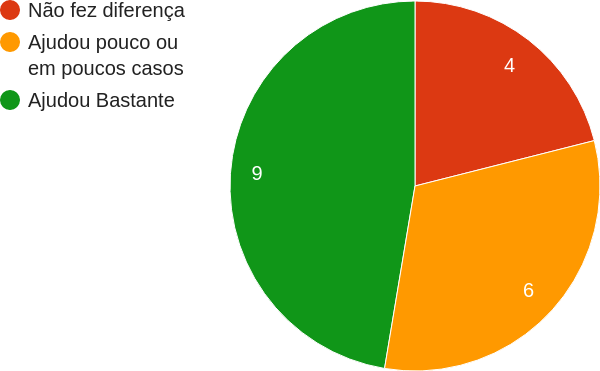
\includegraphics[width=0.50\textwidth]{Grafico-dif.png} 
  \caption{Respostas para a segunda pergunta do questionário.}
  \label{fig:grafsegperg}
\end{figure}

Nenhum usuário respondeu que os parâmetros dificultaram a busca. Houve uma divisão entre aqueles consideraram o sistema útil e aqueles que não identificaram muitas vantagens em seu uso. Novamente, dado que o sistema tem poucos documentos e as consultas têm um baixo \emph{recall}, talvez a diferença entre as listas de resultados não fosse tão perceptível.

Na terceira pergunta, queríamos saber se os usuários colocariam ou retirariam algum parâmetro. 9 responderam que não fariam modificações. Outros 7 deram algumas sugestões. Muitas envolviam acessibilidade e transporte, como ``horário de funcionamento'', ``número de vagas'' e ``estacionamento/transporte público próximos''. Apenas 1 usuário respondeu que retiraria o parâmetro ``qualidade'', por achá-lo pouco confiável em um aplicativo tão novo. 

A quarta e última pergunta pedia a opinião dos usuários quanto a lista de resultados e se nela faltavam informações. As respostas eram semelhantes a da questão anterior, com alguns itens novos como: ``opção de reserva'', ``aceita vale refeição'', ``música ao vivo''.

Para os trabalhos futuros, essas duas últimas questões são relevantes, pois mostram necessidades dos usuários que não são atendidas. Algumas dessas sugestões já são implementadas em outros sistemas, como o Kekanto ou o GoogleMaps.

Por fim, deixamos um campo para comentários, caso as pessoas quisessem comunicar algo que não estava nas perguntas. Recebemos algumas críticas quanto ao layout do aplicativo e alguns erros que aconteceram. Por exemplo, a aplicação não funcionou corretamente em dispositivos móveis.

Um dos comentários criticava o ranqueamento dos resultados, pois eles não eram totalmente reordenados. Portanto, o sistema de ponderamento pode não ter ficado claro para alguns usuários. Algumas mudanças de layout poderiam ajudar nesse sentido.